%\documentclass{article}
\documentclass[a4paper,12pt]{article}
% Seitenränder in schön für Steven
\usepackage[paper=a4paper,left=25mm,right=25mm,top=25mm,bottom=25mm]{geometry}
\usepackage{enumitem}
\usepackage{amsmath}
\usepackage{float}
\usepackage{graphicx}
\usepackage{tikz}
\usepackage{titling}


% Schusterjungen und Hurenkinder bestrafen
\clubpenalty50000
\widowpenalty50000
\displaywidowpenalty=50000

% Buchstaben mit kringel drum: %
\newcommand*\mycirc[1]{%
	\begin{tikzpicture}[baseline=(C.base)]
	\node[draw,circle,inner sep=1pt](C) {#1};
	\end{tikzpicture}}

\newcommand*\red[1]{\textcolor{red}{#1}}

\author{Benedict Hans, Christoph Dollase, Steven Te\ss endorf}
\setlength{\droptitle}{-5em} % set the title to the top of the page

% ==========================
% ===== START HERE!! =======
% ==========================
\title{ \textbf{Problem Sheet 10}}
\setcounter{section}{10} % Nummer des Aufgabenblattes

\begin{document}	 
	\maketitle	 %Some Vodoo-magic
	
	\subsection{CSMA/CD}
	\begin{enumerate}[label=(\roman*),itemsep=0pt]
		\item \textbf{What is a collision?}
		\begin{itemize}[itemsep=0pt]
			\item  happens when two frames are transmitted simultaneously
			\item  both frames overlap and the signals are garbled
			\item  all messages are destroyed
			\item  frames will be retransmitted after a random time
		\end{itemize}
		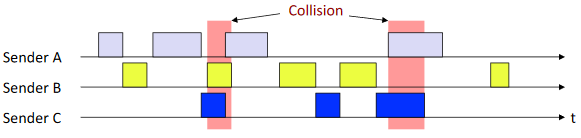
\includegraphics[width=0.8\linewidth]{collision.png}
		\item \textbf{What does Carrier Sense mean?}
		\begin{itemize}[itemsep=0pt]
			\item  stations can sense channel and tell whether it is busy or not
			\item  if busy: stations don't start with transmissions
		\end{itemize}
		\item \textbf{What does the term persistence mean?}\\
		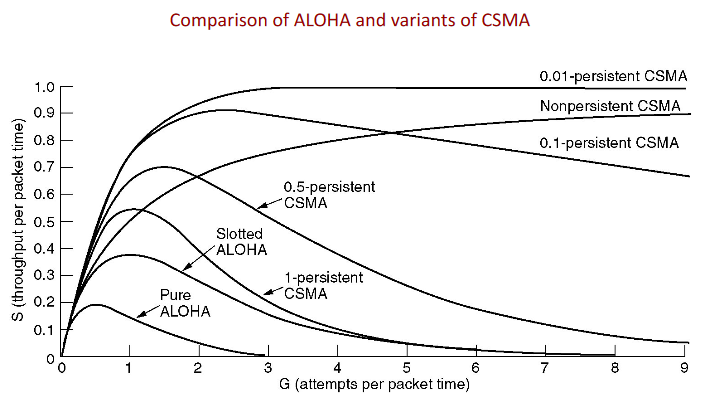
\includegraphics[width=0.75\linewidth]{csma.png}
		\begin{itemize}[itemsep=0pt]
			\item 1-persistent CSMA
			\begin{itemize}[itemsep=0pt]
				\item  when a station has data to send, it first listens to the channel
				\item  if channel is busy, station waits until it becomes idle
				\item  when channel is idle, station transmits a frame
				\item  if collision happens, station waits a random amout of time and starts all over again
				\item  1- persostent $\Rightarrow$ station transmits with probability of 1 if channel is idle		
			\end{itemize}
			\item Non- persistent CSMA
			\begin{itemize}[itemsep=0pt]
				\item  if channel is busy, station waits a random time, repeats algorithm
			\end{itemize}
			\item p- persistent CSMA
			\begin{itemize}[itemsep=0pt]
				\item  applied in slottet channels (slotted ALOHA)
				\item  if channel is on idle, station transmits with probability p in current slot and with probability (1-p) it defers until next slot
				\item  if next slot is on idle, station again transmits with probability p and defers with (1- p) 
			\end{itemize}		
		\end{itemize}
		\item \textbf{Consider a channel with only a few stations that all have a low sending propability. Which type of persistence would be most effective?}
		\begin{itemize}[itemsep=0pt]
			\item 1- persistent CSMA, probably
		\end{itemize}
		\item \textbf{Consider a channel with a huge number of stations that transmit frequently. Which type of persistence would lead to better channel utilization?}
		\begin{itemize}[itemsep=0pt]
			\item p- persistent CSMA, probably
		\end{itemize}
	\end{enumerate}
	
	\subsection{Binary Exponential Backoff}
	\textbf{In the Ethernet specification (IEEE  802.3) a collision causes the Binary Exponential Backoff algorithm to start, in order to resolve the conflict. The algorithm is specified in the specificationas follows:
	\textit{The delay is an integral multiple of the slot time. The number of slot times to delay before the n-th retransmission attempt is chosen as a uniformly distributed random integer r in the range	$0 <= r <= 2^K$  where $K = min(n, 10)$.} In an IEEE 802.3 LAN with 4 stations the following transmission attempts (slots) are given: \\
	\textcolor{blue}{Station A: 1, 3, 12 |  Station B: 1, 7, 8 | Station C: 5 | Station D: 5 }\\
	Frames are buffered till the transmission was successful. The stations are using a function for generating random numbers for the waiting time, which produces values between 0 and 16383. Modulo division is used for restricting the values to the current interval - e.g. after the second conflict it is divided modulo 4, after the third collision modulo 8, etc. The stations’ sequences of random values are given as follows (not all of them are needed here):
	\begin{itemize}[itemsep=0pt]
		\item Station A: 394, 5453, 13815, 4410, 2883, 6402
		\item Station B: 777, 2407, 9599, 3037, 5034, 99
		\item Station C: 1258, 3547, 733, 688, 9234, 2487
		\item Station D: 944, 386, 7427, 4434, 2348, 4287
	\end{itemize}
	Fill in the following table by marking the time slots with an S for successful sending attempts, with an X for a collision, with a W if a station has to wait because of its waiting time, and with a - if a station is inactive, i.e. it has nothing to send.}

	\begin{table}[h!]
		\begin{tabular}{|l|*{20}{p{0.3cm}|}} \hline
			\textbf{Slot} &   1 & 2 & 3 & 4 & 5 & 6 & 7 & 8 & 9 & 10 & 11 & 12 & 13 & 14 & 15 & 16 & 17 & 18 & 19 & 20 \\ \hline
			Station A &    &   &   &   &   &   &   &   &   &    &    &    &    &    &    &    &    &    &    &  \\ \hline
			Station B &    &   &   &   &   &   &   &   &   &    &    &    &    &    &    &    &    &    &    &  \\ \hline
			Station C &    &   &   &   &   &   &   &   &   &    &    &    &    &    &    &    &    &    &    &  \\ \hline
			Station D &    &   &   &   &   &   &   &   &   &    &    &    &    &    &    &    &    &    &    &  \\ \hline
		\end{tabular}
	\end{table}

	
	\subsection{Collision Detection and Frame Size}
	\textbf{Consider a 10 MBit/s CSMA/CD LAN with a bus topology of 50 m. The signal propagates with $2 \cdot 10^8$ m/s in the medium. Calculate the upper bound of the collision detection time. Calculate the minimum frame length that is required to detect a collision.\\}
	
	Worst case: station A senses a free medium and starts to transmit
	\begin{itemize}[itemsep=0pt]
		\item Station B senses a free medium and starts to transmit just at the time the signal from A arrives at B
		\item Signal from B has to travel through the whole network before A can detect the collision
		\item Maximum time until collision detection is twice the signal progagation time
	\end{itemize}

	$t = 2 \cdot \frac{bus~length}{signal speed} = 2 \cdot \frac{50 m}{2 \cdot 10^8 m/s} = 5 \cdot 10^{-7} s$ \\
	\\
	To ensure that the stations are able to detect a collision, the frame be at least $t = 5 \cdot 10^{-7}$ seconds on the medium.\\
	\\
	$frame length_{min} ~/~ bit~rate > t \Rightarrow frame length_{min} > bit~rate \cdot t\\
	frame length_{min} > 10Mbps \cdot 5 \cdot 10^{-7}s \\
	frame length_{min} > 10 \cdot 10^6 bps \cdot 5 \cdot 10^{-7} \\
	frame length_{min} > 5 bit $
	
	\subsection{Multiple Access Effectiveness}
	\textbf{Consider a bus with ten stations. Construct scenarios where the following Multiple Access strategies are efficient or inefficient, respectively, in terms of medium utilization.}
		\begin{enumerate}[label=(\roman*),itemsep=0pt]
		\item \textbf{TDMA}
		\begin{itemize}[itemsep=0pt]
			\item 
		\end{itemize}
		\item \textbf{CSMA/CD}
		\begin{itemize}[itemsep=0pt]
			\item 
		\end{itemize}
		\item \textbf{Bitmap Protocol}
		\begin{itemize}[itemsep=0pt]
			\item 
		\end{itemize}
	\end{enumerate}
	
\end{document}

% Hier nach passiert nichts mehr, daher nutzen wir das als kleines Cheat-Sheet ;)
% ===============================================================================

% Aufzählungen (auch merhstufig):
\begin{itemize}[itemsep=0pt]
	\item 
\end{itemize}

%Bilder eifnügen:
\begin{figure}[h!] %h! sorgt dafür dass das Bild möglichst nicht woanders hingeschoben wird
	%Erklärung: [width=0.5\linewidth] -> Bild ist maximal so breit wie die Hälfte des Schriftbildes
	\includegraphics[width=0.5\linewidth]{Bildname.jpg} 
	\caption{Bildunterschrift}
\end{figure}

%Tabelle einfügen:
\begin{table}[h!] %h! sorgt dafür dass die Tabelle möglichst nicht woanders hingeschoben wird
	\caption{Tabellenüberschrift}
	%hinter {tabular}: Anzahl Spalten (c=center, l=linksbündig, r=rechtsbündig, | Spaltenstriche)
	\begin{tabular}{|c|c|c} 
		A & B & C  \\ % \\ = return (neue zeile)
		\hline % horinzontale Linie
		0 & 1 & 2
	\end{tabular}
\end{table}
